\providecommand{\main}{../../..}
\documentclass[\main/main.tex]{subfiles}
\begin{document}

\subsection{Esercizio 6}
Si deve decidere se introdurre misure restrittive alle importazioni per difendere l'industria nazionale.

Se non si fa niente, le perdite stimate in un'opportuna unità di misura saranno pari a 20. Se invece si procede a introdurle, le nazioni concorrenti potrebbero rispondere con misure leggere (con una probabilità stimata del 30\%) oppure pesanti (con una probabilità del 70\%).

Nel primo caso, si otterrebbe un guadagno complessivo di 100, nel secondo si dovrà decidere se sostenere una guerra commerciale oppure no. Se si rinuncia, le perdite saranno di 30. Se ci si imbarca in una guerra commerciale c'è una probabilità del 50\% di vincerla (con un guadagno di 50) oppure di perderla (con una perdita di 70).

Si disegni l'albero decisionale per la decisione basata sull'ottimizzazione del guadagno atteso e si determinino la strategia ottima.

\subsection{Soluzione esercizio 6}

\subsubsection*{Albero di decisione}
\begin{figure}
  \begin{tikzpicture}
    \Tree[.root
    [.\text{misure protezioniste}
    [.\text{$70\%$ misure pesanti}
      [.\text{sostengo guerra commerciale}
        [.\text{$50\%$ vinco guerra} [.$50$ ]]
        [.\text{$50\%$ perdo guerra} [.$-70$ ]]
      ]
      [.\text{rinuncio guerra commerciale} [.$-30$ ]]
    ]
    [.\text{$30\%$ misure leggere} [.$100$ ]]
    ]
    [.\text{libero mercato} [.$-20$ ] ]
    ]
  \end{tikzpicture}
\end{figure}

\begin{figure}
  \begin{tikzpicture}
    \Tree[.root
    [.\text{misure protezioniste}
    [.\text{$70\%$ misure pesanti}
      [.\text{sostengo guerra commerciale} [.$-35$ ]]
      [.\text{rinuncio guerra commerciale} [.$-30$ ]]
    ]
    [.\text{$30\%$ misure leggere} [.$100$ ]]
    ]
    [.\text{libero mercato} [.$-20$ ] ]
    ]
  \end{tikzpicture}
  \caption{Step 1: caso medio sostenendo guerra commerciale}
\end{figure}

\begin{figure}
  \begin{tikzpicture}
    \Tree[.root
    [.\text{misure protezioniste}
    [.\text{$70\%$ misure pesanti} [.$-30$ ]]
    [.\text{$30\%$ misure leggere} [.$100$ ]]
    ]
    [.\text{libero mercato} [.$-20$ ] ]
    ]
  \end{tikzpicture}
  \caption{Step 2: scelgo di rinunciare a guerra commerciale}
\end{figure}

\begin{figure}
  \begin{tikzpicture}
    \Tree[.root
    [.\text{misure protezioniste} [.$9$ ]]
    [.\text{libero mercato} [.$-20$ ]]
    ]
  \end{tikzpicture}
  \caption{Step 3: caso medio per le misure di risposta}
\end{figure}

Le misure protezioniste danno il guadagno atteso migliore.

\end{document}
